\clearpage
\subsubsection{MSVC + \olly}
\myindex{\olly}

2 пары 32-битных слов обведены в стеке красным.
Каждая пара --- это числа двойной точности в формате IEEE 754, переданные из \main.

Видно, как первая \FLD загружает значение 1,2 из стека и помещает в регистр \ST{0}:

\begin{figure}[H]
\centering
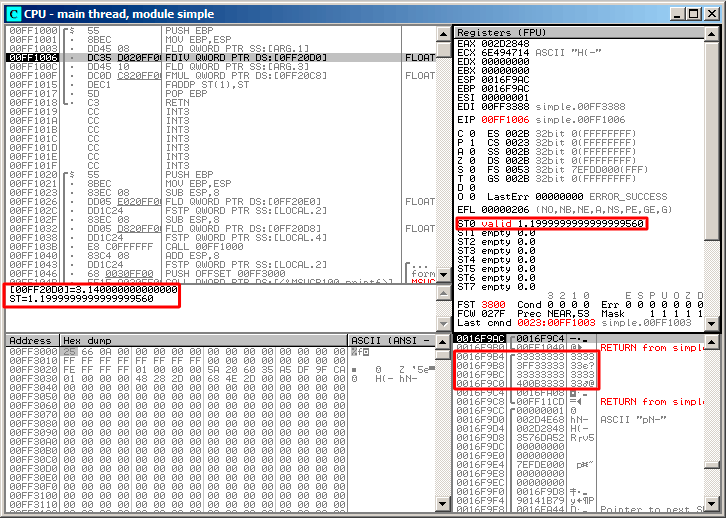
\includegraphics[scale=\FigScale]{patterns/12_FPU/1_simple/olly1.png}
\caption{\olly: первая \FLD исполнилась}
\label{fig:FPU_simple_olly_1}
\end{figure}

Из-за неизбежных ошибок конвертирования числа из 64-битного IEEE 754 в 80-битное (внутреннее в FPU),
мы видим здесь 1,1999\ldots, что очень близко к 1,2.

Прямо сейчас \EIP указывает на следующую инструкцию (\FDIV), загружающую константу двойной точности 
из памяти.

Для удобства, \olly показывает её значение: 3,14.

\clearpage
Трассируем дальше. 
\FDIV исполнилась, теперь \ST{0} содержит 0,382\ldots
(\gls{quotient}):

\begin{figure}[H]
\centering
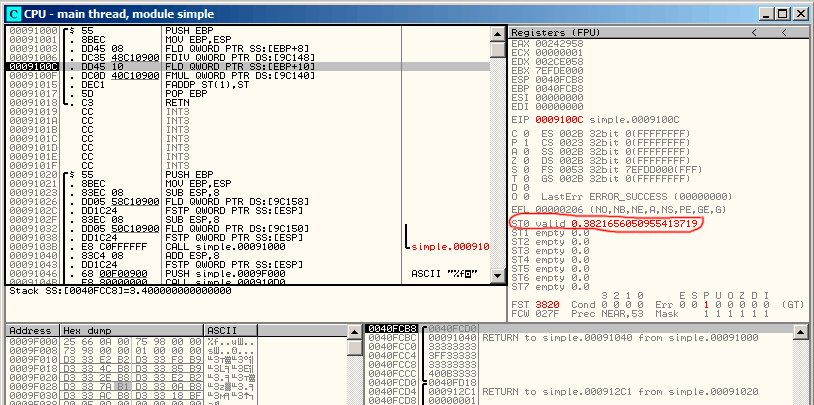
\includegraphics[scale=\FigScale]{patterns/12_FPU/1_simple/olly2.png}
\caption{\olly: \FDIV исполнилась}
\label{fig:FPU_simple_olly_2}
\end{figure}

\clearpage
Третий шаг: вторая \FLD 
исполнилась, загрузив в \ST{0} 3,4 (мы видим приближенное число 3,39999\ldots): 

\begin{figure}[H]
\centering
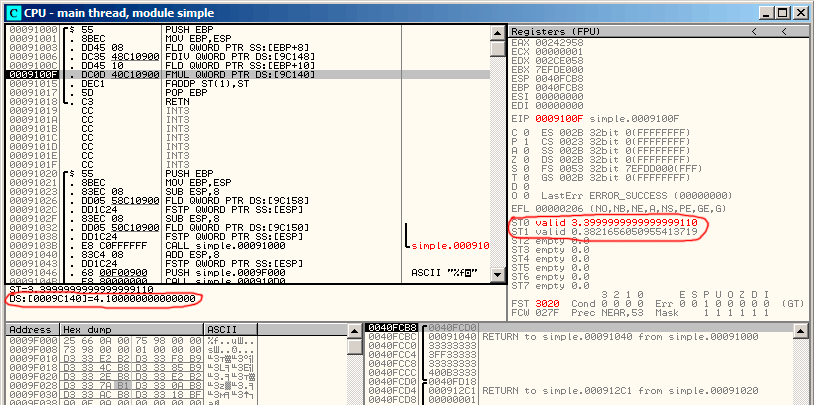
\includegraphics[scale=\FigScale]{patterns/12_FPU/1_simple/olly3.png}
\caption{\olly: вторая \FLD исполнилась}
\label{fig:FPU_simple_olly_3}
\end{figure}

В это время \gls{quotient} \IT{провалилось} 
в \ST{1}.
\EIP указывает на следующую инструкцию: \FMUL. 
Она загружает константу 4,1 из памяти, так что \olly тоже показывает её здесь.

\clearpage
Затем: \FMUL исполнилась, теперь в \ST{0} произведение:

\begin{figure}[H]
\centering
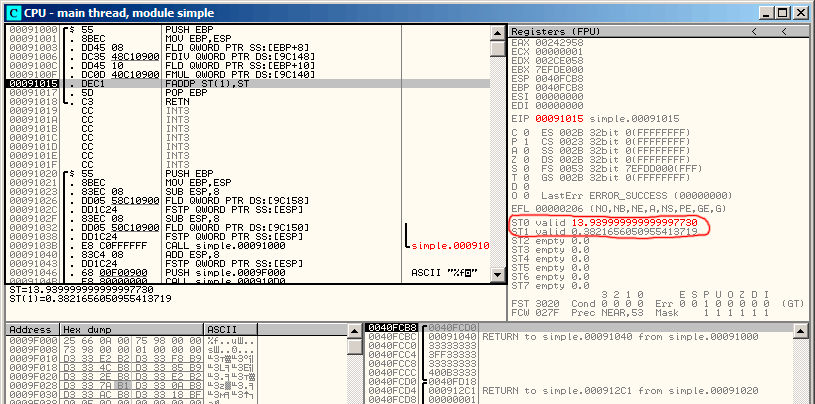
\includegraphics[scale=\FigScale]{patterns/12_FPU/1_simple/olly4.png}
\caption{\olly: \FMUL исполнилась}
\label{fig:FPU_simple_olly_4}
\end{figure}

\clearpage
Затем: \FADDP исполнилась, теперь в \ST{0} сумма, а \ST{1} очистился:

\begin{figure}[H]
\centering
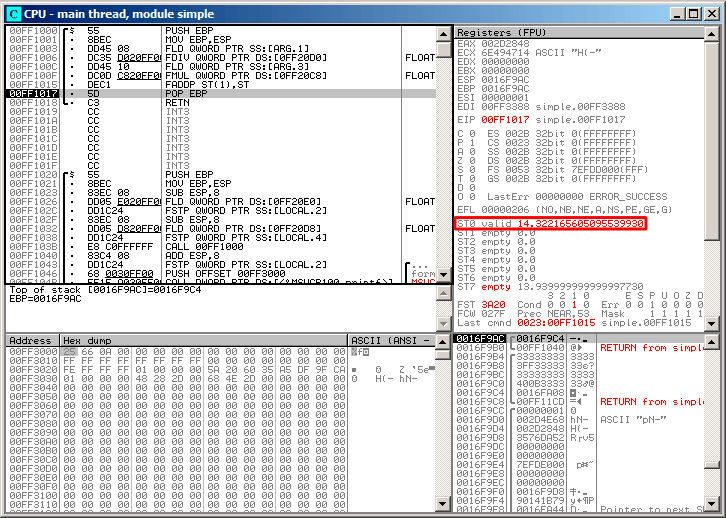
\includegraphics[scale=\FigScale]{patterns/12_FPU/1_simple/olly5.png}
\caption{\olly: \FADDP исполнилась}
\label{fig:FPU_simple_olly_5}
\end{figure}

Сумма остается в \ST{0} потому что функция возвращает результат своей работы через \ST{0}.

Позже \main возьмет это значение оттуда.

Мы также видим кое-что необычное: значение 13,93\ldots теперь находится в \ST{7}.

Почему?

\label{FPU_is_rather_circular_buffer}
Мы читали в этой книге, что регистры в \ac{FPU} представляют собой стек: \myref{FPU_is_stack}. 
Но это упрощение.
Представьте, если бы \IT{в железе} было бы так, как описано. Тогда при каждом заталкивании (или выталкивании) в стек,
все остальные 7 значений нужно было бы передвигать (или копировать) в соседние регистры, 
а это слишком затратно.

Так что в реальности у
\ac{FPU} есть просто 8 регистров и указатель (называемый \GTT{TOP}), содержащий номер регистра,
который в текущий момент является \q{вершиной стека}.

При заталкивании значения в стек регистр \GTT{TOP} меняется, и указывает на свободный регистр. 
Затем значение записывается в этот регистр.

При выталкивании значения из стека процедура обратная. Однако освобожденный регистр не обнуляется
(наверное, можно было бы сделать, чтобы обнулялся, но это лишняя работа и работало бы медленнее).
Так что это мы здесь и видим. 
Можно сказать, что \FADDP сохранила сумму, а затем вытолкнула один элемент.

Но в реальности, эта инструкция сохранила сумму и затем передвинула регистр \GTT{TOP}.

Было бы ещё точнее сказать, что регистры \ac{FPU} представляют собой кольцевой буфер.

